\chapter{Architecture of CMU Sphinx-4 as an Example of a typical ASR}
\label{chap:sphinx}
 \section {Overview} 
CMU Sphinx represents a classical speech recognizer, including the following
main components: frontend, decoder and knowledge base with language and acoustic
models and dictionary. In the next sections the components of the speech
recogniser are analysed in more details.
 
 \begin{figure}[htbp]
  \centering
    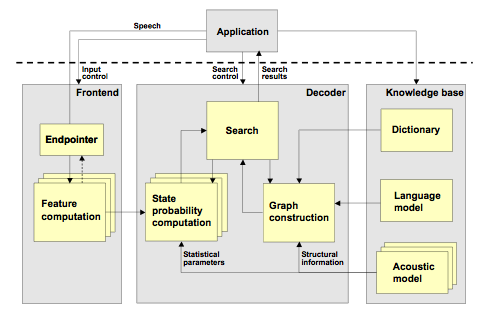
\includegraphics[width=1.0\textwidth]{images/sphinxarch.png}
 \caption{Sphinx-4 Architecture Overview \parencite
 {Lamereetal2013:Eurospeech}.}
  \label{fig:sphinx arh}
\end {figure}

 \section {Acoustic Analysis} 

Frontend computes feature vector \textit {Y } - representation of a speech
signal, using acoustic analysis.  It provides methods for manipulating the data processors, performing
specific transformation functions on input data \parencite{Lamereetal2013:Eurospeech}.

In a physical sense human speech is a sound wave, characterized by a particular amplitude, frequency, period and length.
Decoding is preceded by features extraction and digitalizing of a signal in such a way, that mathematical operations and calculations are made possible. 

Preprocessing of speech as an analogous signal demands the following steps. First, the waves are sampled, which allows getting a discrete signal from the 
continuous one. Second, the samples are quantized, mapping the analog values to digitalised ones. Third, a digital signal is converted to its 
spectral representation, applying a short-time Fourier transform. The resulting sound spectrum contains the amount of vibration at each individual frequency. 
Figure \ref {fig:spectro} shows a wave form, pitch contour, spectral
representation and transcription with alignment of the phrase \textit {ich danke
 Ihnen und wir sehen uns dann}.
\begin{figure}[htbp]
  \centering
    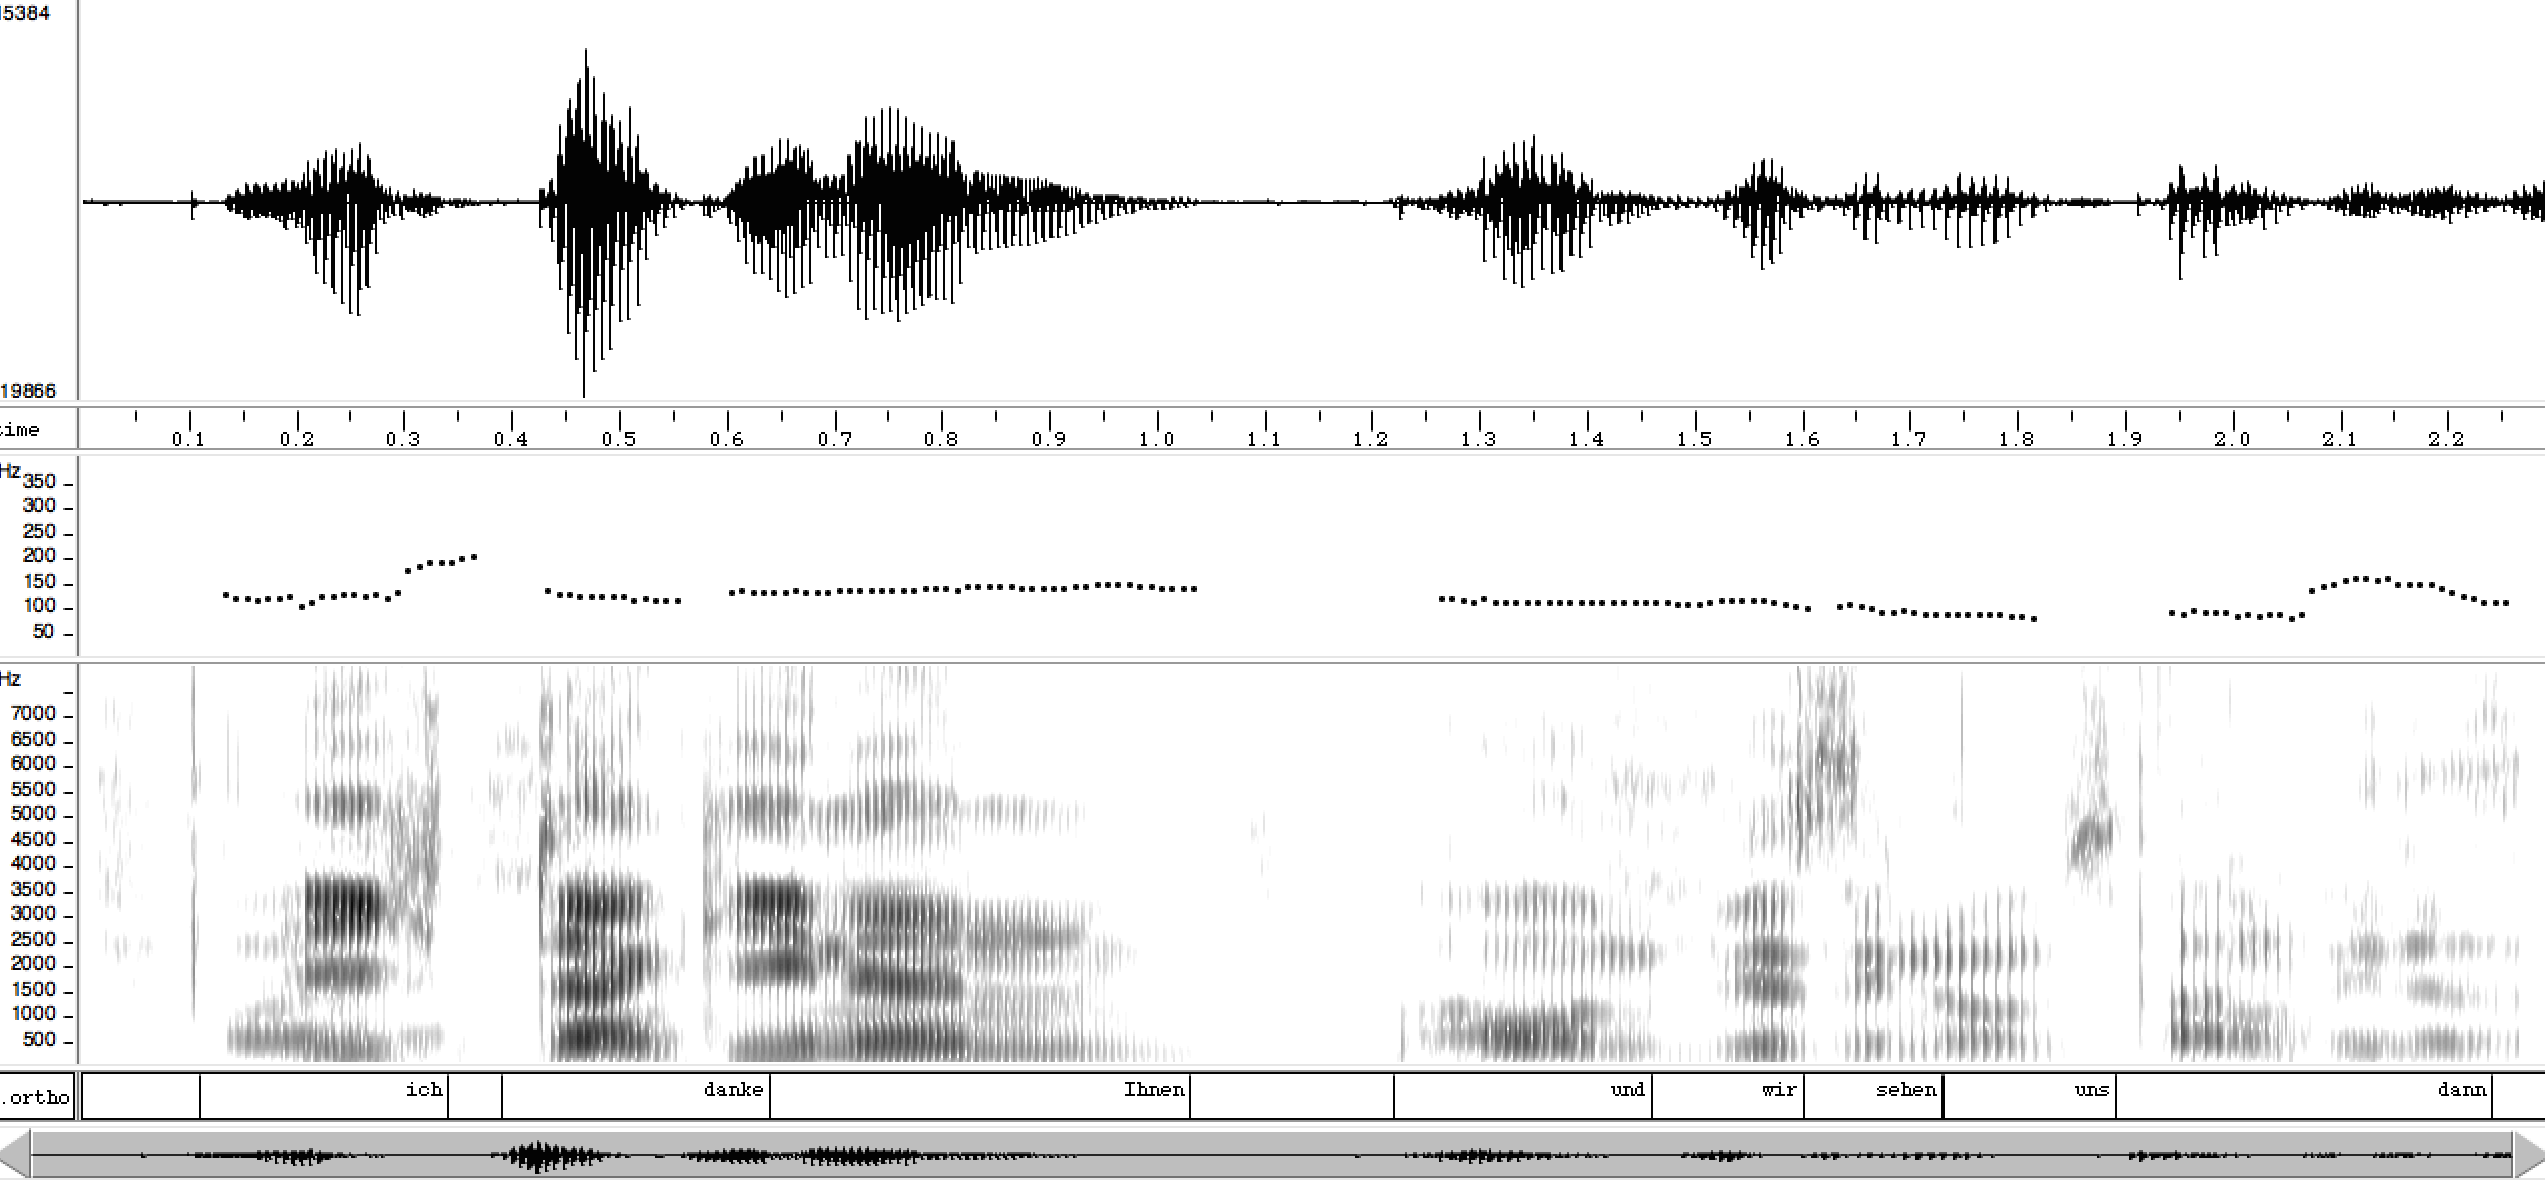
\includegraphics[width=1.0\textwidth]{images/spectro.png}
 \caption{From the top of the figure: an acoustic waveform, pitch contour,
 spectrogram and transcription with gold alignment of the phrase \textit {ich
 danke Ihnen und wir sehen uns dann}. }
  \label{fig:spectro}
\end {figure}

Finally, with the help the sound spectral representation acoustic vectors of
features Y are created. One of the most commonly used for this purpose method is a mel frequency
cepstrum (MFC). This method calculates coefficients representing the amplitudes
of the resulting spectrum, so-called mel frequency cepstrum coefficients (MFCC).
Resulting acoustic vectors of features are used as a representation of a sound waveform, forwarded to the decoder for recognition  \parencite
{jurafskymartin2009}.

\section {Acoustic Model} 

Acoustic model finds out the probability for an observing an acoustic vector
\textit {Y } given a sequence of words \textit {P (Y|W)}. Theoretically, for a
small vocabulary it can be found by sampling several variants of the words and computing statistical similarity of the inputs with 
the existing samples. However, when the vocabulary is very large we have to move
down to the level of word subunits or phonemes.

Acoustic model contains statistical representation of each phoneme in the form a Hidden
Markov Models (HMM), which abstracts the physical process of pronouncing of a
particular phoneme. An example HMM is depicted in the figure \ref
{fig:onehmm}. This HMM for phoneme recognition has 3 states S0, S1, S2. Letters
’A’ shows the transition probabilities within the states, ’B’ - output probabilities, ’Y’ -observations.  Sphinx-4 is a typical
HMM-based speech recognizer with 3 and 5 states HMMs 
\parencite {jurafskymartin2009}. 

\begin{figure}[htbp]
  \centering
    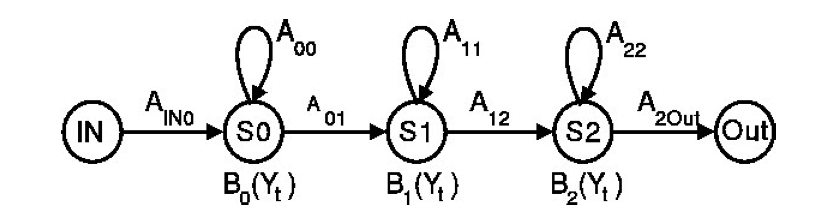
\includegraphics[width=1.0\textwidth]{images/one_hmm.png}
 \caption{A typical HMM abstraction \parencite {jurafskymartin2009}. }
  \label{fig:onehmm}
\end {figure}

Word representations in acoustic model form a network of HMMs. Acoustic models
are created from an hours-long audio recordings and their corresponding transcriptions. In order to
get a statistical representation of phonemes, i. e, build a HMM for each
phoneme, the speech corpus data is subjected to the training process.
Speech corpus data and resulting models differs in speech parameters: microphone speech, broadcast speech, conversational speech, 
telephone speech. Too general 
models are not applicable for more specific language conditions, whereas too specific models are limited in its usage. The right 
choice of the acoustic model 
increases performance of a recogniser. To match specific conditions of an application an acoustic model model should be trained respectively, providing
enough training data is available.


\section {Language Model} 

Language model describes the probability of a word in a speech sequence \textit
{Y } {P (W)} and attempts to predict the next word in a sentence, depending on
the prior context.
Language models are based on n-gram sequences of words, where the number of words of
the prior context is equal n-1. Language models are built on the basis of an
application corpus \parencite {jurafskymartin2009}. Depending on the
application, language models can be either generalized or domain specific. 

%\lstinputlisting[firstline=117753,
% lastline=117763]{images/Cocolab_Verbmobil.lm}




%\captionof{lstlisting}{The first 100 lemmata}
Sphinx-4 uses two types of language models:  statistical and grammar-based ones.
Statistical language model describes the probability of a word in a speech
sequence (P (W)) and attempts to predict the next word in a sentence, depending on the prior context.
Language models are based on n-gram sequences of words, where the number of words of the prior context is equal n-1. The most widely used sequence is tri-gram. 
An extract from a statistical language model is shown in the figure \ref
{fig:lm} .
%Symbols <s> and </s> means the start and the end of an utterance respectively,
% and the figures - the probability of a trigram occurrence.

 \begin{figure}[htbp]
  \centering 
 
% \lstdefinestyle{nonumbers} 
 %{numbers=none}  
%\begin{lstlisting}[style=nonumbers]
\begin{lstlisting}[frame=single]
...
\data\
ngram 1=4604
ngram 2=38548
ngram 3=80671
...
\3-grams:
...
-0.0512 wir sehen uns 
-0.7566 wir senden Ihnen 
-1.0576 wir sicher fertig 
-1.0576 wir sicher im 
-0.7566 wir sicherlich was 
-1.3587 wir sie den 
-1.3587 wir sie doch 
-1.3587 wir sie hier 
-1.3587 wir sie ja 
-0.0941 wir sieben Uhr 
...
\end{lstlisting}
 \caption{An extract from Verbmobil language model for Sphinx-4.}
  \label{fig:lm}
\end {figure}

Statistical language models are built on the basis of an application corpus.
Corpus contains a list of sentences that are used to train the language model. The best results are achieved, when the model is tuned the 
application speech situation. Statistical language models for telephone
conversations are less effective for robot instructions.

Grammars describe very simple types of languages in Java Speech Grammar Format
(JSGF). The do not contain probabilities, but it is possible to weight
some of the grammar elements.  An example of a simple JSGF grammar for German
digits is shown in the  picture \ref {fig:grammar} .

\begin{figure}[htbp]
  \centering 
 \lstset{
  literate={ü}{{\"u}}1
}
%  \lstdefinestyle{nonumbers} 
%  {numbers=none}  
%\begin{lstlisting}[style=nonumbers]
\begin{lstlisting}[frame=single]
grammar digits;

public <numbers> = ( eins | zwei | drei | vier | fünf |
 sechs |sieben | acht | neun | null) * ;

\end{lstlisting}
 \caption{JSGF grammar for German digits from one to ten.}
  \label{fig:grammar}
\end {figure}

Here also some words about Aligner Grammar for forced-alignment. 

\section {Dictionary} 

Pronunciation dictionary belongs to the knowledge base of Sphinx-4. It is made
of all occurred in the application words and their transcriptions. Pronunciation dictionary is used by the decoder during word identification as a reference. 
A typical transcription file is shown in the figure \ref {fig:dic}.
\newline
\begin{figure}[htbp]
 % \centering 
\lstset{literate=%
  {Ö}{{\"O}}1
  {Ä}{{\"A}}1
  {Ü}{{\"U}}1
  {ß}{{\ss}}2
  {ü}{{\"u}}1
  {ä}{{\"a}}1
  {ö}{{\"o}}1
}
%  \lstdefinestyle{nonumbers} 
%  {numbers=none} 
%  
%  
% %\begin{center}
% %\begin{lstlisting}[style=nonumbers]
\begin{lstlisting}[frame=single]
spezifizieren	S p e t s i f i t s i: 6 n  
grenz	g r E n t s 
sechsund	z E k s U n t
Malediven	m a l e d i: v @ n
Gemütlicheres	g @ m y: t l I C @ r @ s
lau	l aU
zugereicht	t s u: g @ r aI j t
vornehmer	f o: 6 n e: m 6
gereist	g @ r aI s t
Südfrankreich	z y: t f r a N k r aI C
zerteilen	t s E 6 t aI l n
\end{lstlisting}
 \caption{An extract from the dictionary file. For correspondence between
 Sphinx-4 representation and German phonemes see appendix \ref{chap:appA}. }
  \label{fig:dic}
\end {figure}
\newline
The dictionary can be maid manually according to transcription conversions, or
alternatively using generators. Some words in the dictionary can have several possible transcriptions. On the other hand, differently written words 
may sound identically (compare homophones TO and TWO). Difference between the homophones is only evident within context. Distinction of, for 
example, such homophones as ice-cream vs. I scream, real eyes vs. realize vs. real lies, addressed mail vs. a dressed male, etc. is a really 
challenging task for an ASR, especially when the context is not clear.

Words that are not in the dictionary are not recognized in Sphinx. So it is
necessary either to use an extended dictionary, containing the missing words or to use 
sphinx  grapheme to phomene converter g2p, which automatically generates
pronunciations for missing words, based on pronunciation rules.  

% On the basis of acoustic model, language model and dictionary the search graph
% is build, which is used by the decoder together with the frontend information
% to determine the most probable output sequence. Decoder
% traverses the network of HMM states and finds the path with the best
% score, using Viterbi algorithm. 
 
%\section {Search Graph and Linguist}
\section {Decoder}
Speech recognition decoder receives data from acoustic inputs, acoustic and
language models and returns the most probable word sequence. The task that the decoder is solving can be
formulated in plain text as follows:
\begin {center}
\textit {What is the most likely sentence out of all
sentences W in the language L given some acoustic input Y? }
\end {center}
In the terms of mathematics we are dealing with an optimisation problem,
formulated with a Bayes decision rule \parencite {jurafskymartin2009}:
\[w_opt = argmax P(W|Y ) = \frac {P(Y |W)P(W)} {P(Y)} = argmax P(Y |W)P(W)\]

Decoder solves the above optimisation problem, involving complicated search algorithms. One of the most commonly used for speech recognition algorithm is 
Viterbi algorithm. Viterbi is a dynamic programming search algorithm. It traverses the network of HMM states and 
finds the path with the best score.

\begin{figure}[htbp]
  \centering
    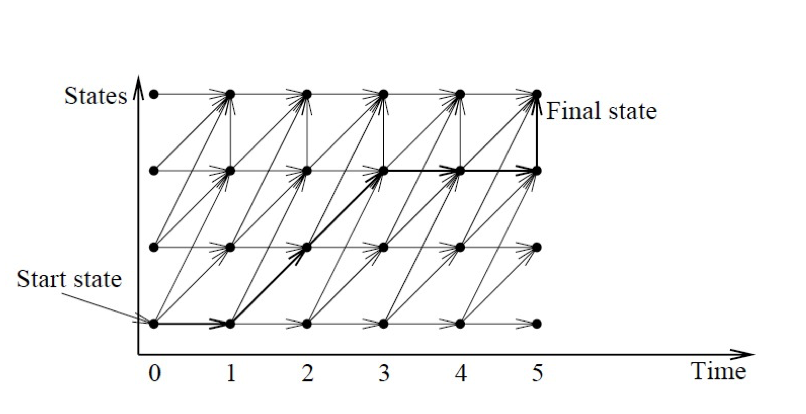
\includegraphics[width=1.0\textwidth]{images/viterbi.png}
 \caption{Viterbi search as dynamic programming \parencite
{Ravishankar96efficientalgorithms}.}
  \label{fig:hmm}
\end {figure}

Abstract representation of the Viterbi algorithm is shown in the in the figure 4.7. One axis represent states in the HMM network, another time.
 Arrows means transitions through the network. Each point in this 2-D space represents the best path probability for the corresponding state at that time. 
 Every state has a best predecessor and starting from the final state and using backtracking it is possible to find the best path sequence for the whole search.
Complexity of Viterbi algorithm is equal $\mathcal{O}(N2T)$, where N
is the total number of states and T is the total duration \parencite
{Ravishankar96efficientalgorithms}. In Sphinx-4 Viterbi search is implemented as
\textit {token passing algorithm} \parencite {Young89Token}. 

\section {Search Graph and Linguist} 

Search graph and linguist are the central components of the decoder search
module.  The linguist is responsible for representing and managing the search
space for the decoder. The role of the linguist is to provide, upon request, the search graph that is to be used by the decoder.
The linguist is a generic interface that provides language model services.

Search graph is build in Sphinx-4 by Linguist on the basis of acoustic
model, language model and dictionary. When the grammar or language model is changed the
search graph is updated.  An example of the search graph for the words ``one''
and ``two'' is shown in the figure \ref{fig:hmm}.

\begin{figure}[htbp]
  \centering
    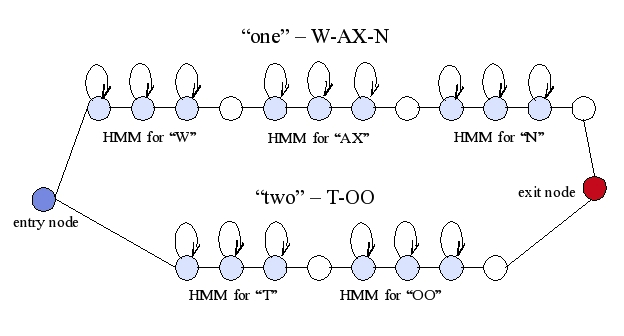
\includegraphics[width=1.0\textwidth]{images/hmm.png}
 \caption{An example search graph for the words ``one'' and ``two''.}
  \label{fig:hmm}
\end {figure}

The main types of Linguist in Sphinx-4 are: flat linguist, dynamic flat linguist
and lex tree linguist. 

\subsection {Flat Linguist} 
\subsection {Dynamic Flat Linguist} 
\subsection {Lex Tree Linguist} 









